\section{Parser}

\begin{frame}[fragile]
	\frametitle{Parser - Operatoren Priorität}
	\begin{lstlisting}
%right in
%right ASSIGN ADD ...
%right QUESTIONMARK COLON
%left OR
...
%nonassoc LESSER GREATER LESSER_EQUAL...
...
%nonassoc INCREMENT DECREMENT
	\end{lstlisting}
\end{frame}

\begin{frame}[fragile]
	\frametitle{Struktur Happy File}
	\begin{lstlisting}[basicstyle=\tiny]
		
Program
    : Class                { [$1] }
    | Program Class        { $1 ++ [$2] }
    | Program SEMICOLON    { $1 }

Statement
    : SingleStatement SEMICOLON             { $1 }
	...
    | IF LEFT_PARANTHESES Expression RIGHT_PARANTHESES
        Statement ELSE Statement
                                            { If $3 $5 (Just $7) }
    | IF LEFT_PARANTHESES Expression
        RIGHT_PARANTHESES Statement
        %prec THEN                          { If $3 $5 Nothing }
    | Switch                                { $1 }
	\end{lstlisting}
\end{frame}

\begin{frame}[fragile]
	\frametitle{Beispiel}
	\begin{lstlisting}[language=Java, basicstyle=\tiny]
class SimpleIf {
	int i;
	void doIf() {
		int a;
		a = 5;
		i = 0;
		if(a < 5) {
			i = a;
		}
		else {
			i = 2;
		}
	}
}
	\end{lstlisting}
	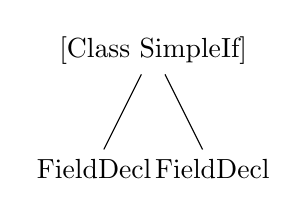
\begin{tikzpicture}
		\node(class){[Class \enquote{SimpleIf}]}
			child { node { FieldDecl } }
			child { node { FieldDecl } }
			;
	\end{tikzpicture}
\end{frame}
